%%%%%%%%%%%%%%%%%%%%%%%%%%%%%%%%%%%%%%%%%%%%%%%%%%%%%%%%%
%
% Autore: Cristian Di Pietrantonio
% 16 aprile 2016
% Nota: questa è una semplice trascrizione della lezione del 5 aprile dove si inizia a parlare del model checking.
% Sebbene segua il discorso del professore in maniera coerente, il modo in cui sono scritti non è ottimale. Ci possono
% essere errori grammaticali o sviste.
% Il codice a cui si fa riferimento è presente nella repository uni_verifica-validazione nella cartella
% model-checking/dfs-tronci
%
%%%%%%%%%%%%%%%%%%%%%%%%%%%%%%%%%%%%%%%%%%%%%%%%%%%%%%%%%%
\documentclass[a4paper, 11pt]{article}
\usepackage{geometry, graphicx}
\usepackage[utf8]{inputenc}

\title{Model checking}

\begin{document}
\maketitle

\textbf{NOTA}: è una trascrizione di una registrazione, potrebbero esserci errori ortografici e pezzi mancanti. \\

 L'ultima volta è stato visto lo schema generale per risolvere la \emph{reachability} con la dfs. Ora bisogna applicarlo al nostro contesto. Si presentano subito due problemi:
 \begin{itemize}
  \item nello schema si è assunto un numero finito di stati. Non è cosi nei modelli di sistemi cyber-fisici;
  \item non abbiamo una forma chiusa per l'evoluzione del sistema, nel senso che, ad esempio, se si prende un programma basta eseguirlo, la parte fisica va risolta, quindi ci serve un solver. Va aggiustato tale schema per questa soluzione.
 \end{itemize}

 Per quanto riuarda la dinamica, si usa un simulatore. Non è l'unico approccio. Invece di usare un simulatore, si tratta solamente i sistemi i sistemi chiusi (tipicamente lineari) e si verificano con model checker (una verifica matematica). Ha il suo senso restringersi ai modelli lineari perche all'inizio si astrae molto il modello. Tuttavia nei sistemi ciberfisici non può essere una soluzione, in quanto la parte fisica è bel lontana dall'essere lineare; inoltre se si vuole entrare a ``gamba tesa'' in un progetto (ossia verificare un sistema gia fatto), quello non può essere rifatto da zero per renderlo lineare(fattore di lavoro e costo). Alla fine il modello finale è di dettaglio e quindi sicuramente non lineare: come quando si astrae il codice con gli automi per verificare i requisiti, ma il target è il codice e bisogna concentrarsi (per quanto riguarda la verifica) su quello.

 Si procede allora dividendo il ``mondo'' in tre sottosistemi:
 \begin{itemize}
  \item Il sistema da verificare;
  \item Il monitor che dice se le possibili evoluzioni del sistema rispettano le specifiche;
  \item Un modello dell'ambiente;
 \end{itemize}

 Il sistema da verificare è considerato fisso (gia prodotto). Il modello dei disturbi (provenienti dall'ambiente) invece lo si può modellare liberamente; qualunque sia il sistema da verificare si può assumere che tra un disturbo e l'altro vi sia un tempo finito e che i disturbi siano presi da un pool finito. Se si fanno queste due ipotesi, a questo punto la possibili sequenze di disturbi sono finite. Quindi il sistema non è finito, ma lo sono le sequenze di disturbi. A questo punto quello che si può fare è sfruttare questa proprietà per terminare la ricerca.\\


Si può immaginare il \emph{plant} (ndr: in realtà il plant è solo la parte fisica) come un sistema di load-balancing ed $x$ è il carico (carico computazione ad esempio), noise e failures sono l'ambiente che modifica il carico, ed $u$ è il controllo che tenta di mantenere il carico costante (mantenere un certo indicatore di errore vicino allo 0). Se siamo sopra stiamo facendo overprovisioning, e non va bene, e se stiamo sotto non forniamo abbastanza carico. Si può immaginare che sia un sistema di controllo della temperatura, allora $x$ è la temperatura, noise e failures cambiano la temperatura, e u controlla la temperatura. La dinamica è semplice (lineare) per facilitare l'esempio.\\
La derivata di $x$ è $ax$, l'equazione rappresenta ciò che il sistema farebbe di moto proprio. Con la $u$ ci si oppone ai disturbi dell'ambiente, impiegando un controller. [sempre in system.mo] Questo controller è un classico, si chiama PID (propotional integrative derivative). Funziona introducendo il concetto di errore, che è la differenza tra quello che si desidera e tra quello che succede. Si desidera la $x$ a 0, quindi l'errore è $0 - x$. Dopodiche si fa un azione $u$ che è proporzionale all'errore con una costante $k_0$. Poi c'è la parte ``integrative''. Quello che vorrei che l'azione sia proporzionale all'integrale del'errore. Invece di scrivere l'integrale, scriviamo $der(z) = 0 - x$, in modo tale che $z$ è l'integrale dell'errore. Allora aggiungiamo $k_1 \cdot z$ ad $u$; l'ultima parte è ``derivative'', quindi mettiamo $k_2 \cdot der(x)$. I PID saranno sempre così, e il punto sta nello scegliere i valori giusti per $k_0$, $k_1$ e $k_2$. Nell'esempio attuale sono stati dati (tirati fuori dal taschino, con valori 100, 10, 10). \`E stata fatta un azione energica, quindi, perche più quei valori sono alti più la $u$ è aggressiva. Quindi, quello presentato, è il SUV (system under verification).\\

Ora ci serve un monitor. Il monitor osserva il sistema; in questo caso misuriamo ed osserviamo lo stato. Non è ovvio che si possa fare, ma in questo caso facciamo finta di si. Dopodiché tira fuori un valore booleano per dire se va bene o meno. Qui è implementato come un segnale che inizialmente è false, poi appena c'è un errore va a true e resta a true. Il monitor è la variabile $y$, $x$ è l'input e ragiona nel seguente modo. $x$ voglio sia a 0, o vicino a 0, con una certa tolleranza. Si inizializza nel sistema la $x$ ad $1$. Quello che voglio testare è quanto ci mette il mio controllore a portarmi dove deve portarmi, cioè in questo caso a 0 (l'errore). Uno dei parametri fondamentali è il setup time che è il tempo che ci metto a ridurre l'errore sotto la soglia. Quindi appena si accende il sistema non è detto che il mondo ``sia nella norma'', ma dopo una certa soglia di tempo l'errore deve essere portato sotto la soglia consentita. C'è un campionameno ogni T secondi. Ad ogni campionamento ci si chiede: se prima si stava a true, oppure il valore assoluto di $x$ è maggiore della soglia ed il tempo è maggiore di uno, allora metti a true. Se $y$ era a true resta a true per sempre. Questa è la forma tipica di un monitor. La proprietà tipicamente voglio che valga da un certo tempo in poi (il sistema deve avere il tempo di setup).\\

Ora si vedranno i due modi per modellare l'ambiente in Modelica (con le funzioni di input). Si ha il sistema, il monitor e l'ambiente (di cui ancora deve parlare). Si deve creare un sistema chiuso collegando le componenti. Questo è fatto in un altro file (ClosedSystem.mo); il monitor è agganciato attraverso $x$ al sistema, dopodiché invece usare il modello dell'ambiente vogliamo usare una proprietà di modelica che è di mettere un input direttamente dalla simulazione (dal file .py). Definiamo due variabili reali in input, failures e noise, e devo agganciarli al sistema. [vedi Esempi in classe/03 - loadbalancer] Modelica ha due modi per dare in input funzioni al modello: tramite, appunto, funzioni oppure tramite matrici con i dati. Per passare funzioni, in questo caso noise e failures, bisogna fare un vettore con le funzioni: nello script di python creiamo una funzione (input\_function), che ha come parametro sempre il tempo, e che torna un array con le due funzioni (ossia una sequenza di valori reali). Dopodiché bisogna legare queste funzioni al nome delle variabili del modello, e lo si fa creando un \emph{input\_object}; questo oggetto è una tupla il cui primo elemento è un vettore con i nomi delle variabili, e il secondo elemento è una funzione del tempo che mi ritorna un array di funzioni, tante quanti sono i nomi nell'array. [viene eseguito il modello]

\begin{center}
 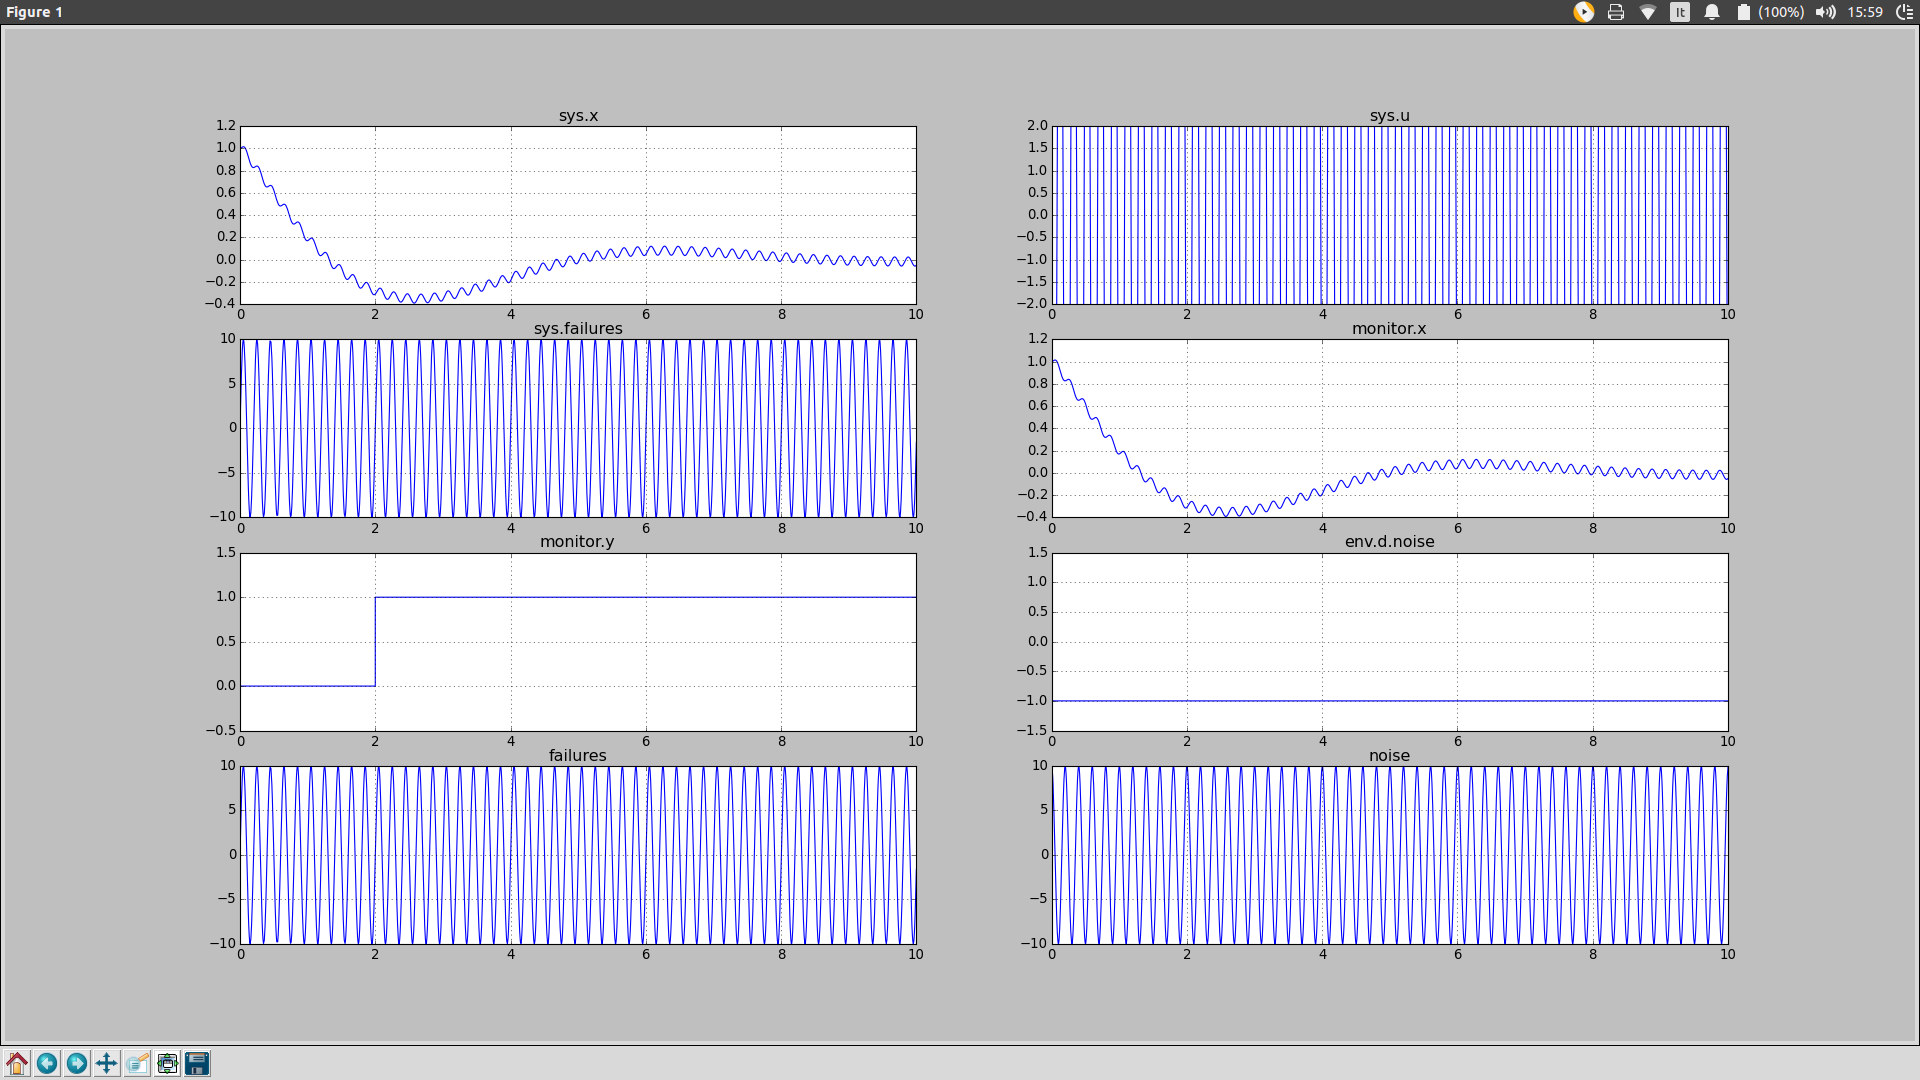
\includegraphics[width=350px]{png/00-loadbalancer.png}
\end{center}

Nel caso dell'input passato tramite matrici, viene costruita una matrice $M$ che ha la prima colonna contenente una serie di punti che rappresentano istanti temporali (nel nostro caso ugualmente distanziati) (quindi un punto per riga); vi è poi una colonna per ogni input (che è sempre in funzione del tempo) da passare al modello, con il valore $i$-esimo preso all'istante $M[0][i]$ (in altre parole una riga ha come primo elemento il tempo in cui sono stati misurati i successivi elementi, che sono i valori dell'input). Per creare le colonne dell'input da mettere nella matrice sono state create due funzioni, $func1$ e $func2$. A questo punto, creata $M$, la si passa al simulatore come prima tramite un oggetto.\\

A questo punto si passa alla fase successiva. Abbiamo il solito sistema con il solito monitor, ma utilizziamo il nostro modello dell'ambiente (invece di passare l'input a runtime). Come si modella l'ambiente in maniera non doterministica? Con un simulatore ho sistemi deterministici ma l'ambiente non lo è. Si fa creando un automa che accetta il linguaggio definito dall'ambiente. In altre parole ho un automa che analizza la seguenza di disturbi in input e mi dice se è ammissibile o no. Se arrivo ad uno stato non ammissibile, ogni prolungamento di quella sequenza non è ammissibile (il duale è che se una sequenza è ammissibile, ogni suo prefisso deve esserlo). [enviroment.mo] Questo è un automa che è cloccato, chiaramente i disturbi sono distanziati da un quanto di tempo che si decide (è u parametro); dopodiche si hanno 4 variabili di stato. Una è il valor medio (le sequenze di disturbi che il valor medio è 0, per semplicità si disturba solo la noise). Un altra variabile è $adm$, che dice se la sequenza è ammissibile, un intero $N$ che dice quanti disturbi si sono visti fino a quel momento, e poi si ha la profondità della sequenza. Poi si hanno i disturbi (noise e failures); Dopo ci i crea lo stato. Modelica ha il tipo record. Ci si crea un record i cui elementi sono le variabili di stato del modello dei disturbi. Poi ci si crea un altro record dove si hanno i distrurbi ``impacchettati''. Con questi due record ci si dichiara i disturbi e due stati (input, output). Ora siamo pronti per definire l'automa. Bisogna definire la funzione di transizione, che è deterministica; infatti non è l'automa che genera il successivo disturbo, ma è l'automa che dice se un nuovo disturbo ci piace o meno. La funzione ritorna un nuovo stato. L'automa evolve leggendo un disturbo e calcolo la next() (non si può fare la pre di un record, quindi si chiama su ogni elemento del record).\\

Ora si aggancia tutto in System-close.mo. Bisogna organizzare la simulazione in modo tale da esplorare tutte le possibili sequenze di disturbi ammissibili. \`E qui che si fa la DFS. Dichiariamo una classe Search.py. Innanzitutto ci serve un hashtable e uno stack (dove mettere la sequenza esplorato); servono un insieme di funzioni che parlano con il simulatore (che chiamano il metodo next()). Ci si crea anche uno stato del modello. A questo punto lo stato è lo stato dell'intero sistema. C'è la questione di individuare le variabili che determinano lo stato. Nei sistemi continui sono tipicamente quelle di cui si fa la derivata. Ci potrebbero essere situazioni più omplicate dove il sistema non è in forma normale (con roba algebrica) e ci sono derivate di variabili che non fanno parte dello stato.\\

Viene avviata quindi la ricerca e si creano gli elementi dello stack. Il tempo diventa parte dello stato quindi si crea una tupla per incorportarlo alle altre informazioni e si spinge tutto sullo stack. L'altra cosa che va messa nello stack è l'azione iniziale (stiamo considerando la prima chiamata); qui sorge una differenza con la search generale vista la volta scorsa (nella quale si metteva dopo lo stato ogni possibile azione, mentre qui solo una). Qui si mette una sola azione perché si vuole andare in ordine lessicografico e mi devo ricordare, al ritorno, dove stavo. [continua a descrivere il codice in search.py]
\end{document}
